\documentclass[11pt]{article}

% Change "review" to "final" to generate the final (sometimes called camera-ready) version.
% Change to "preprint" to generate a non-anonymous version with page numbers.
\usepackage{acl}

% Standard package includes
\usepackage{times}
\usepackage{latexsym}

% For proper rendering and hyphenation of words containing Latin characters (including in bib files)
\usepackage[T1]{fontenc}
% For Vietnamese characters
% \usepackage[T5]{fontenc}
% See https://www.latex-project.org/help/documentation/encguide.pdf for other character sets

% This assumes your files are encoded as UTF8
\usepackage[utf8]{inputenc}

% This is not strictly necessary, and may be commented out,
% but it will improve the layout of the manuscript,
% and will typically save some space.
\usepackage{microtype}

% This is also not strictly necessary, and may be commented out.
% However, it will improve the aesthetics of text in
% the typewriter font.
\usepackage{inconsolata}

%Including images in your LaTeX document requires adding
%additional package(s)
\usepackage{graphicx}

\title{Project 1}

\author{Jesus Soto Gonzalez \\
  \texttt{jhsoto@iastate.edu}}

\begin{document}

\maketitle

\begin{abstract}
This first project for COM S 5790, Natural Language Processing applies basic NLP and word embedding methods 
to a given dataset. We preprocessed the text by tokenizing it, removing stopwords, and using phrase mining. 
From this, we created frequency- and TF--IDF-based word clouds to highlight key terms. 
For semantic analysis, we trained Word2Vec models on both words and phrases to find the nearest neighbors 
of top TF--IDF terms. Phrase mining with \texttt{gensim}'s bigram and trigram models helped capture multiword 
expressions and produced clearer, more meaningful embeddings.
\end{abstract}

\section{Methods}

\subsection{Preprocessing}
The dataset was first filtered to only include abstracts with Category = 1. 
Each abstract was sentence-split, tokenized, lowercased, and cleaned by removing stopwords and non-alphabetic 
tokens using NLTK. The result was saved both as plain text for word clouds and as token lists in JSON for 
Word2Vec tasks respectively. This step ensured consistency across all later tasks and reduced noise 
from irrelevant or low value tokens.

\subsection{Phrase Mining}
To capture multiword terms, I used the \texttt{gensim} library for phrase mining. 
I first trained a bigram model on the tokenized corpus with a minimum count of 8 and a threshold of 8.0. 
This combined pairs of words that often appeared together. 
Then, I trained a trigram model on top of the bigrams to join longer expressions. 
In both cases, phrases were written with underscores, such as \textit{carcass\_composition}, 
\textit{average\_daily\_gain}, and \textit{backfat\_thickness}.  

I also tested different parameter values. 
Stricter settings 10, 10.0 created fewer but very strong phrases, while looser ones 5, 5.0 or 3, 3.0 
created more phrases but added noise. The balanced setting 8, 8.0 worked best, since it kept important 
domain phrases like \textit{quantitative\_trait\_locus} and \textit{meat\_quality} without introducing too 
many random ones. This choice was important because phrase quality directly influenced the TF--IDF terms 
and the results from Word2Vec.

\subsection{TF--IDF and Word Clouds}
From both the single word and phrased corpus I computed frequency counts and TF--IDF scores. 
The top-ranked terms were visualized as word clouds, which made it easy to compare terms that 
are common against those that are more distinctive. This provided a clear way to see how 
phrase mining and weighting methods highlight different aspects of the corpus.


\subsection{Word2Vec}
I trained Word2Vec models on both the words and phrased corpus using CBOW with a vector size of 100, a window of 5,
and a minimum count of 10 as required. Then, to evaluate the models, I looked at the nearest neighbors of the 
top TF--IDF terms and compared how the results changed when using phrases instead of single words.

\section{Main Results}

\subsection{Word Clouds -- Task 1}
The frequency based word cloud was dominated by very common research terms such as \textit{qtl}, 
\textit{traits}, \textit{study}, and \textit{genes}. These words appear often across many abstracts but do not 
point to specific findings. In contrast, the TF--IDF word cloud highlighted more distinctive domain terms, 
including \textit{ascites}, \textit{earlobe}, \textit{pleurisy}, and \textit{ketosis}. This shows how TF--IDF can 
surface technical vocabulary that is less frequent overall but more informative for understanding the dataset. 

(see Appendix, Figures~\ref{fig:freq_wc_task1} and~\ref{fig:tfidf_wc_task1}).  


\subsection{Word2Vec -- Task 2}
The Word2Vec model was trained on the corpus using CBOW with a vector size of 100, a window of 5, 
and a minimum count of 10. To evaluate the model, I looked at the nearest neighbors of the top TF--IDF terms.  

One clear example was \textit{ascites}, which refers to the buildup of fluid in the abdomen and is often 
used in a disease or health context \citep{clevelandclinic2025ascites}. Its nearest neighbors included 
\textit{death}, \textit{vaccine}, \textit{pathogens}, and \textit{treatment}. These are all directly related 
to illness and medical outcomes, showing that the model was able to group words with a strong connection.  

At the same time, some abbreviations such as 
\textit{lp}, \textit{ifc}, and \textit{su} returned vague neighbors like \textit{become} or \textit{finally}, 
which were harder to interpret and less useful.  

Overall, the results show that Word2Vec found useful connections for biological or health-related 
terms, but it struggled with abbreviations or other terms that did not occur often enough in the dataset.

\subsection{Word Clouds -- Task 3}
Using the phrased corpus, the word clouds showed some multiword expressions that were not visible in Task 1. 
The frequency word cloud still contained mainly common research terms, but now phrases like 
\textit{candidate\_genes} appeared, giving more precise meaning than the single words alone.  

The TF--IDF word cloud highlighted technical phrases, such as \textit{subclinical\_ketosis}. 
Terms like these capture specific meaning that would not have been clear if only individual words were used.  

This improvement was a direct result of the phrase mining experiment in \texttt{phrases.py}, where I tested 
different parameter settings for \texttt{min\_count} and \texttt{threshold}. Looser values produced many 
phrases but also added noise, and stricter values gave very few. The balanced choice (8, 8.0) worked best 
and helped the word clouds show some meaningful scientific terms instead of just single words.  

(see Appendix, Figures~\ref{fig:freq_wc_task3} and~\ref{fig:tfidf_wc_task3}).  

\subsection{Word2Vec -- Task 3}
The Word2Vec model was trained again on the phrased corpus. The same parameters were used: 
CBOW, vector size 100, window size 5, and minimum count 10. I evaluated it the same way as 
in Task 2, by looking at the nearest neighbors of the top TF--IDF terms.  

Some results showed improvements. For example, \textit{ascites} was now grouped with terms or technical 
phrases like \textit{lesions} and \textit{pregnancy\_rate}, which are all linked to health. 
This was more specific compared to the simpler words in Task 2.  

These improvements were possible because of the phrase mining process in \texttt{phrases.py}. Again, the 
balanced parameter setting of (8, 8.0) worked best compared to the others, directly influencing the phrased 
Word2Vec neighborhoods and showing more meaningful connections than in Task 2.  

Even with phrases, not all terms were useful. Abbreviations like \textit{lp} and \textit{ifc} still 
produced neighbors that were hard to interpret, and some words like \textit{abt} were skipped because 
of their low frequency.  

Overall, using the phrased corpus made the neighbors more meaningful by showing technical multiword terms, 
especially in health contexts. However, rare abbreviations and terms were still limiting.  

Finally, I compared all extracted phrases against the trait dictionary using exact string matching. 
Out of 22,719 trait entries, 282 matches were found. When the spaces were replaces with underscores 
to align with the phrased corpus, the number of matches increased to 348. This confirms that a significant 
amount of the phrases overlap with known traits, showing the method captured relevant domain terms.

\vspace*{1em}

Using the ACL template \citep{aclstylefiles}.

\vspace*{1em}

\bibliography{custom}

\vspace*{1em}

\appendix
\section*{Appendix}
\addcontentsline{toc}{section}{Appendix}

\section{ (Word Cloud Figures)}

\begin{figure*}[t]
  \centering
  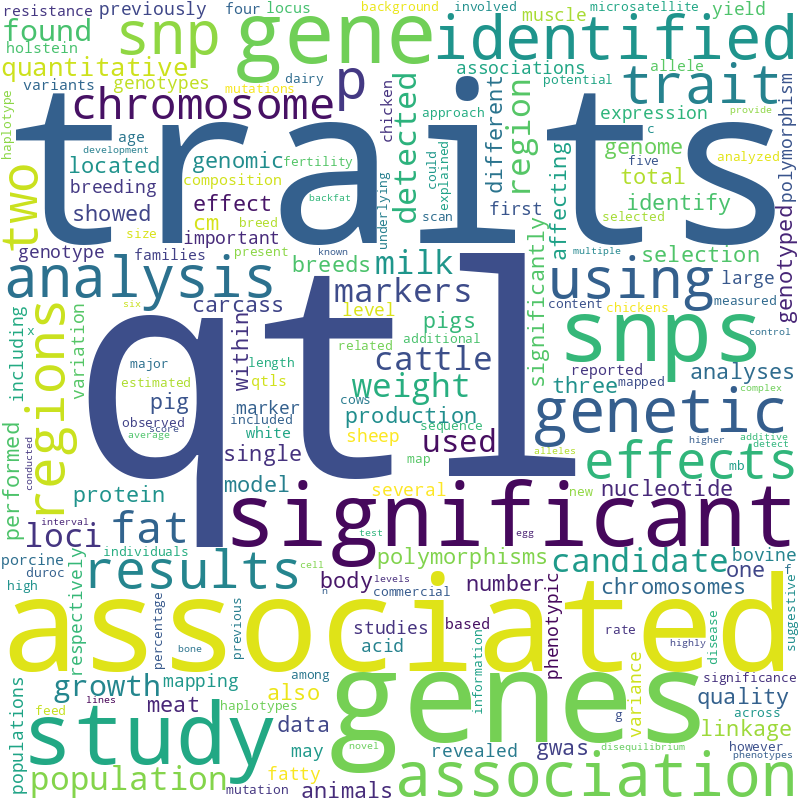
\includegraphics[width=0.48\linewidth]{../outputs/freq_wordcloud_task1.png} \hfill
  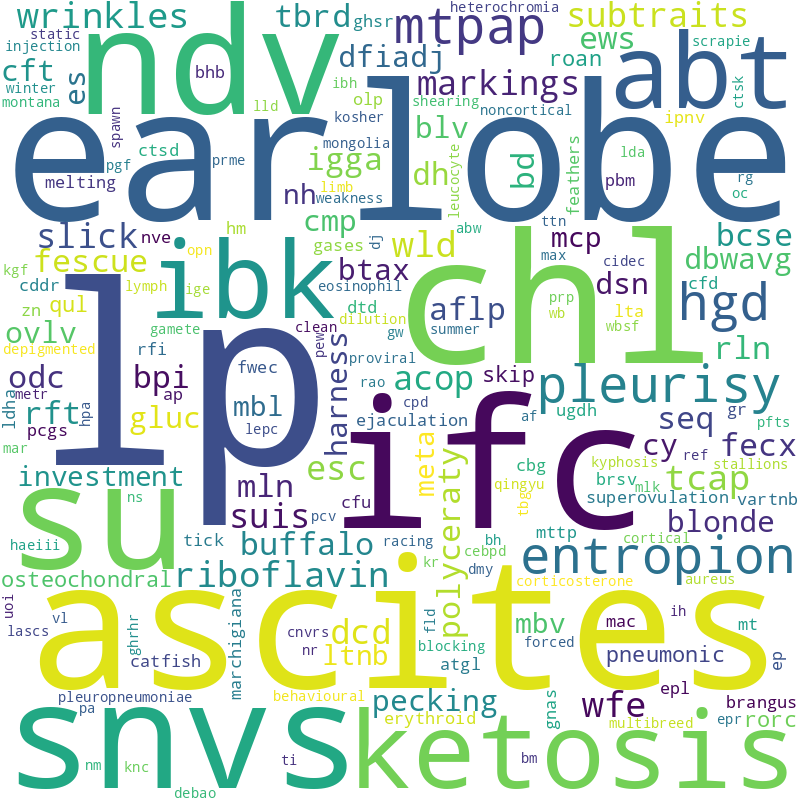
\includegraphics[width=0.48\linewidth]{../outputs/tfidf_wordcloud_task1.png}
  \caption{Task 1 word clouds. Left: frequency-based, showing common terms such as \textit{qtl} and \textit{traits}. 
  Right: TF--IDF-based, highlighting more distinctive terms like \textit{ascites} and \textit{earlobe}.}
  \label{fig:wc_task1}
\end{figure*}

\begin{figure*}[t]
  \centering
  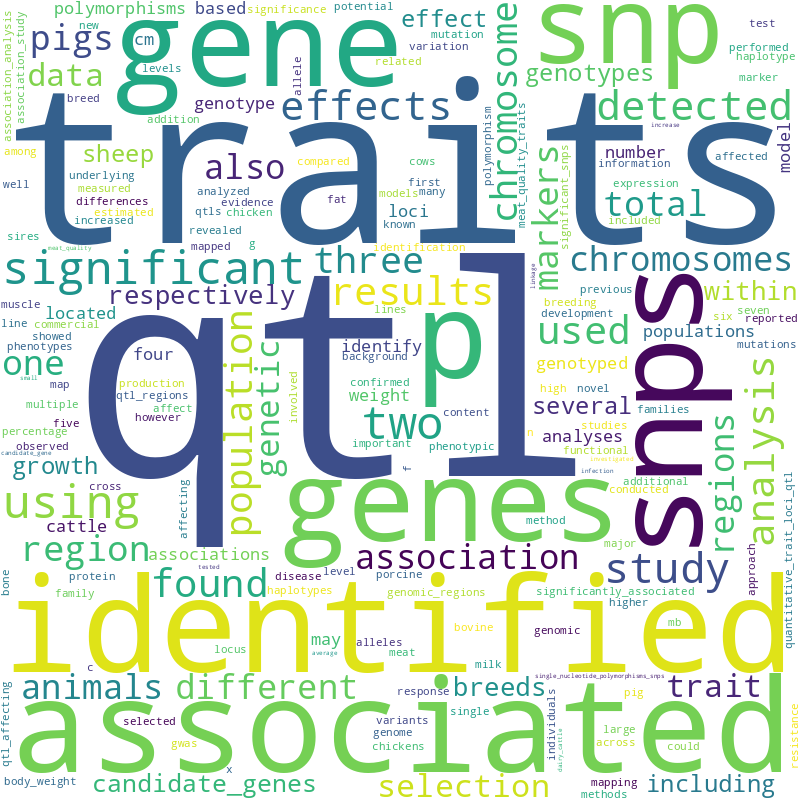
\includegraphics[width=0.48\linewidth]{../outputs/phrased_freq_wordcloud.png} \hfill
  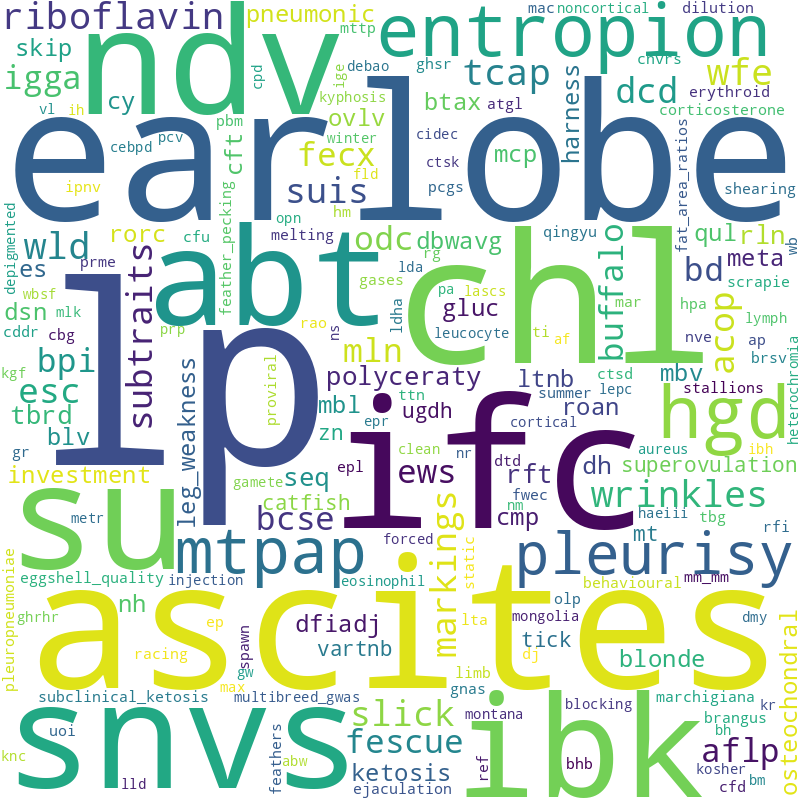
\includegraphics[width=0.48\linewidth]{../outputs/phrased_tfidf_wordcloud.png}
  \caption{Task 3 word clouds with phrase mining. Left: frequency-based, where multiword terms such as 
  \textit{candidate\_genes} appear. Right: TF--IDF-based, highlighting technical phrases like 
  \textit{subclinical\_ketosis}.}
  \label{fig:wc_task3}
\end{figure*}

\end{document}